\section{Introduction}

GLIMMER\footnote{GENIE Land-Ice Model with Multiply Enabled Regions} is the land ice component of GENIE\footnote{Grid-ENabled Integrated Earth-system model}. Its design is motivated by the desire to create an ice modelling system which is easy to interface to a wide variety of climate models, without the user having to have a detailed knowledge of its inner workings. This is accomplished by providing a very well-defined interface, which allows access to all the functionality required by the user. All model fields and time-dependent parameters required by the ice model are passed to it through the argument lists of the supplied subroutines. Initialisation data is supplied through namelist files, while netCDF files are used for platform independent binary I/O. 

GLIMMER is the land-ice component of GENIE, an integrated Earth-system model
being developed as part of the UK e-science initiative, and funded by
NERC. The name GLIMMER stands for Genie Land-Ice Model with Multiply-Enabled
Regions, and its design is motivated by the desire to
create an ice modelling system which is easy to interface to a wide variety of
climate models, without the user having to have a detailed knowledge of its
inner workings. This is
accomplished by providing a very well-defined interface, which allows access to
all the functionality required by the user. All model fields and
time-dependent parameters required by the ice model are passed to it through
the argument lists of the supplied subroutines. Initialisation data is
supplied through easily-understood configuration files, while 
netCDF\footnote{\texttt{http://www.unidata.ucar.edu/packages/netcdf/index.html}} 
files are used for platform-independent binary I/O. Some simple visualisation
code, built on Python, GMT and Proj4 is supplied, although this has not yet
reached a level of functionality to supplant a fully-featured visualisation
and programming environment such as Matlab.

\subsection{What are `Multiply Enabled Regions'?}

The most distinctive feature of the GLIMMER framework is the ability to
run the ice model over several different regions of the globe, and to define
those regions at runtime. Each specified region is termed an \emph{instance}
of the ice model. Primarily, then, GLIMMER provides a uniform interface
between a global climate model and an arbitrary number of ice models. The
processes of downscaling input variables, and subsequently aggregating and
upscaling outputs is handled invisibly by GLIMMER, leaving the user solely
with the tasks of supplying input data and parameters, and handling outputs in
the manner appropriate to the problem being tackled. These techniques could be
applied to any surface model that you might want to run only over
particular regions of the globe.

\subsection{Overview}
GLIMMER consits of two components:
\begin{enumerate}
 \item {\bf GLIDE:} This component is the actual ice sheet model. GLIDE is responsible for calculating ice velocities, internal ice temperature distribution, isostatic adjustment and melt water production.
 \item {\bf Climate Drivers:} GLIDE is coupled to the outside world via two fields describing the ice surface temperatures and mass balance and (optionally) a scalar value for eustatic sea level. These drivers can be derived from simple assumptions, e.g. uniform mass balance or EISMINT tests, or from climate model output, e.g. GENIE or a regional climate model.
\end{enumerate}
These components and how their relations are outlined in Figure \ref{ug.glide}.

\begin{figure}[htb]
 \begin{center}
   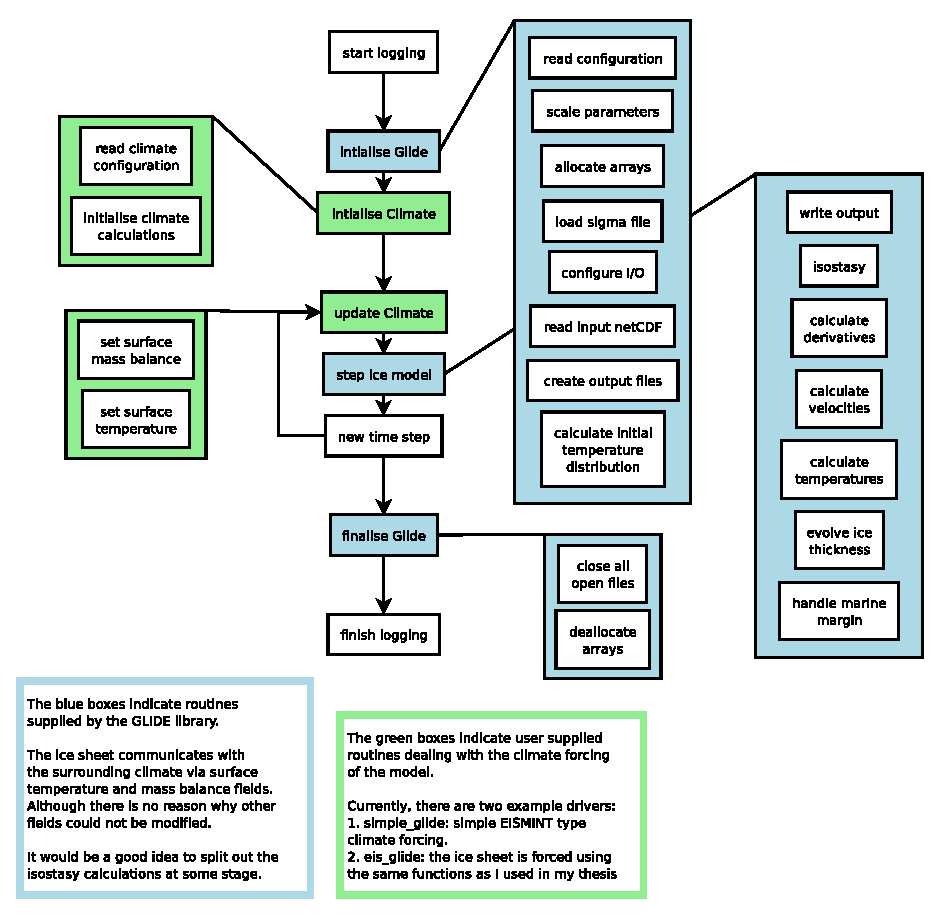
\epsfig{file=\dir/figs/glide.eps,width=0.9\textwidth}
 \end{center}
 \caption{Outline of the GLIDE and Climate components.}
\label{ug.glide}
\end{figure}

Three climate drivers are provided by the GLIMMER module:
\begin{enumerate}
 \item \texttt{simple\_glide}: an EISMINT type driver
 \item \texttt{eis\_glide}: Edinburh Ice Sheet driver. 
 \item \texttt{libglint}: interface to GENIE
\end{enumerate}

\subsection{Configuration, I/O and Visualisation}
Each component is configured using a configuration file similar to Windows \texttt{.ini} files. The model configuration is printed to a log file. 

2D and 3D data is read/written to netCDF files using the CF convention. netCDF is scientific data format for storing multidimensional data in a platform and language independent binary data format. The CF conventions specify the meta data used to describe the file contents.

Many programs can process and visualise netCDF data, e.g. OpenDX. Additionally, the GLIMMER module contains GMT scripts written in Python to visualise the output.

\subsection{Can I use GLIMMER with my climate model?}
We hope so! The external interface of GLIMMER is designed to be quite
flexible, but certain assumptions have necessarily been made about the form
taken by input fields, etc. In general, these are derived from the
characteristics of the GENIE climate model and the Reading IGCM, which is one
of atmospheric models available in GENIE. Nevertheless, the specified input
fields are chosen on the basis of their physical importance, rather than
because of their availability within a given atmospheric model. This may mean
that some pre-processing has to be done before fields may be passed to
GLIMMER, which clearly might have cost implications.

In order to use GLIMMER, the following is necessary:

\begin{itemize}
\item Global input fields must be supplied on a latitude-longitude
  grid. The grid does not have to be uniform in latitude, meaning that
  Gaussian grids may be used. Irregular grids (e.g. icosahedral grids) are not
  supported currently. The boundaries of the grid boxes may be specified; if
  not, they are assumed to lie half-way between the grid-points in lat-lon space.
\item In the global field arrays, latitude must be indexed from north to south
  -- i.e. the first row of the array is the northern-most one. Some
  flexibility might be introduced into this in the future.
\item The global grid must not have grid points at either of the poles. This
  restriction is not expected to be permanent, but in the meantime
  can probably be overcome by moving the location of the polar points to be
  fractionally short of the pole (e.g. at 89.9$^{\circ}$N and 89.9$^{\circ}$S).
\item The user must supply the bedrock topography for each of the ice model
  instances. These data are read from netCDF files.
\item GLIMMER is written in FORTRAN 95, and the Unix/Linux build system
  requires Python, which may be obtained from \texttt{www.python.org}. 
\end{itemize}

Check out the climate drivers for examples of varying complexity.
